\begin{figure}[p]
\centering
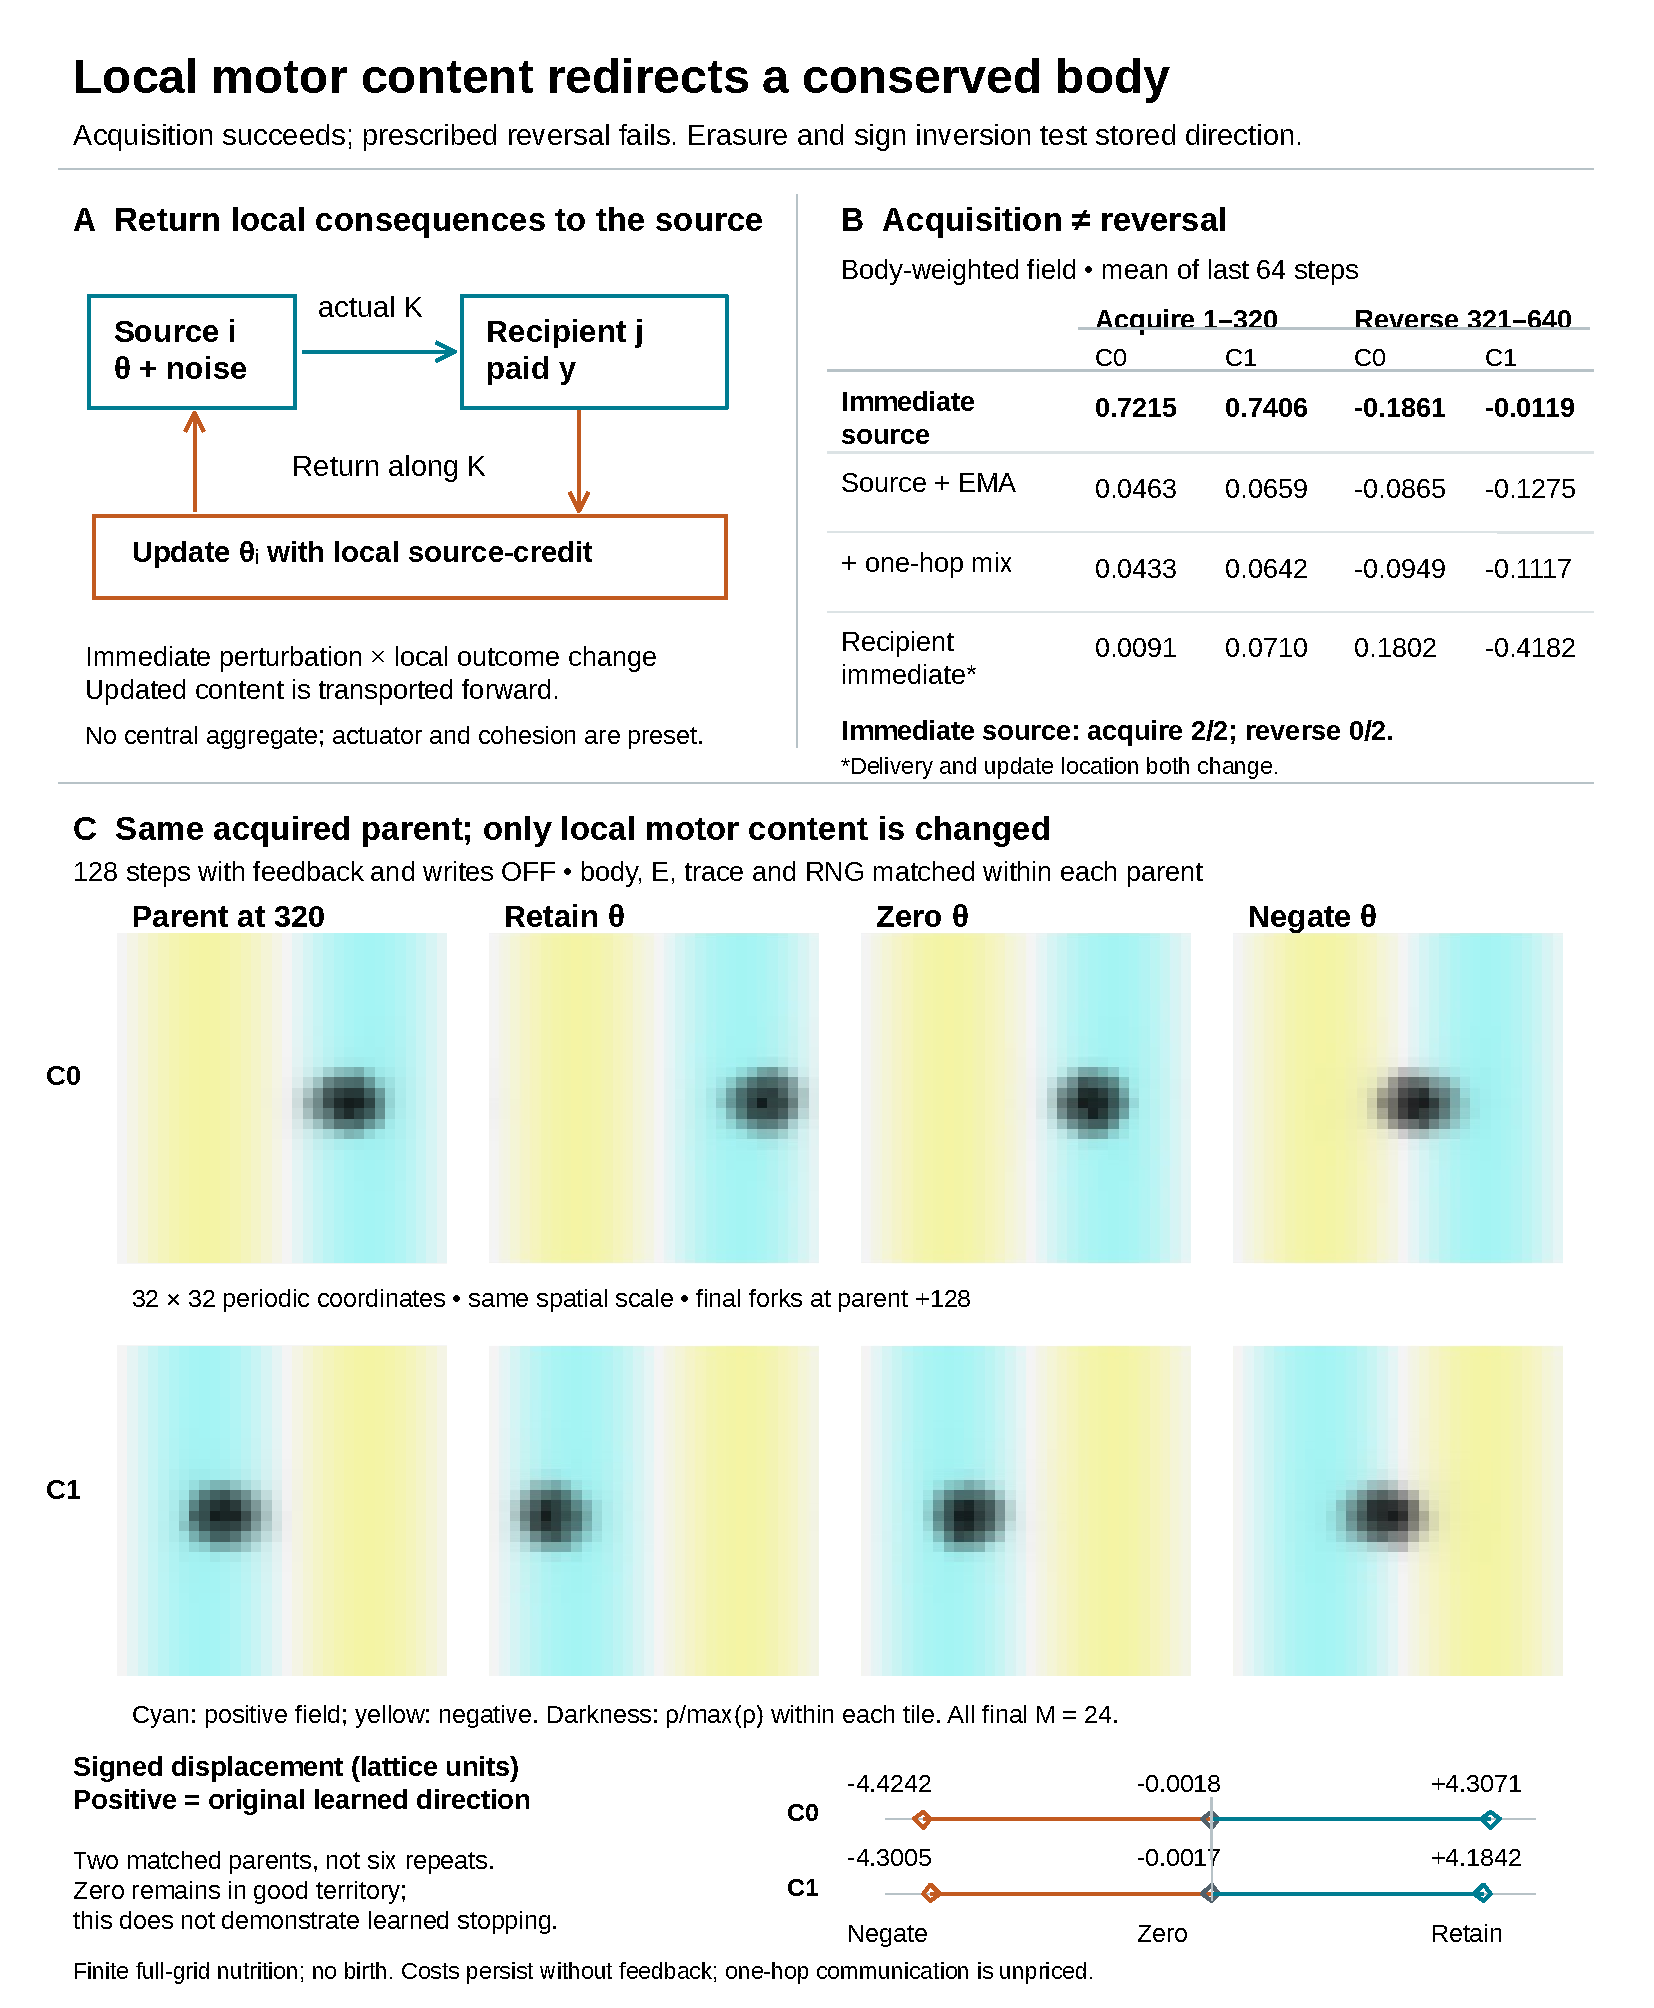
\includegraphics[width=\linewidth,height=0.69\textheight,keepaspectratio]{work/longform_v047/figures/local_motor_v0475/local_motor.pdf}
\captionsetup{font=footnotesize}
\caption{\textbf{Acquired local motor content affects action without successful reversal.}
\textbf{a}, Actually paid local consequences return along executed transport edges to the motor source; updated content travels forward with material. The stochastic actuator and cohesion are supplied, with no central action or reward aggregation. Source and recipient comparisons change both feedback delivery and writing location.
\textbf{b}, The two seed--field conditions acquire a directional bias with the standard immediate source-credit rule but fail the prescribed environmental reversal. Scores are final-64 tissue-weighted field means, not accuracy; the original criterion also requires favourable mass fraction and viability. Tested EMA and neighbour variants do not establish an advantage, and their effective gains are not matched to the immediate rule.
\textbf{c}, Each complete actual-320 parent branches into retained, zeroed and sign-reversed motor content for 128 updates with no payment or new writing. Actual fields retain original coordinates; cyan/yellow denote positive/negative field. Darkness is normalized within each density tile, not a shared absolute-density scale. Signed displacement is measured along each parent's original learned direction. All six futures remain mass 24; zeroed branches retain favourable occupancy and pay less for motion, so almost zero net displacement does not imply learned stopping. These are paired interventions in two parents, not six independent histories. This no-birth local host is distinct from the density-regulated central-action host in Fig.~\ref{fig:young-turnover}; extra one-hop communication and learning arithmetic are unpriced.}
\label{fig:local-motor-content}
\end{figure}
